\documentclass[english]{article}

\usepackage{babel}
\usepackage{graphicx}
\usepackage{times}
\usepackage{pifont}
\usepackage[margin=1in]{geometry}
\usepackage{eurosym}
\usepackage{fancyhdr}

\pagestyle{fancy}
\fancyhf{}
\lhead{Business Model Canvas}
\rhead{Introduction to Business Processes}
\date{}
\setlength\parindent{0pt}

\begin{document}

\title{\vspace{2in}Business Model Canvas\\
\small for EFJ0110 Introduction to Business Processes\\
\vspace{0.5in}
\includegraphics{savonia.jpg}}



\nopagebreak
\maketitle


\vspace{3in}

\author{
\begin{flushright}
Alexey Tukalo,\\
EFA12SF,\\
Information Technology,\\
Savonia University of Applied Sciences
\end{flushright}
}

\date{\today}
\thispagestyle{empty}

\newpage
\setcounter{page}{1}
\setcounter{tocdepth}{2}
\tableofcontents

\newpage

%MAIN CONTENT ******************************************************************************************************************
\section{Introduction}


I think that the best business ideas are created when somebody finds modern solutions
for old usual problems. I do interval running. It is very good kind of fitness, because it
does not take as much time as gym but it allows you to be more active. For ordinary people an interval running is much better than normal running, because any kind of cardio is
effective only if the duration of the training is longer than 40-45 mins, but it is very
difficult to run for so long for the most part of people, that’s why the running intervals
are often mixed with walking ones and it allows to the runner runs longer.
\subsection{Description}
As result of the advantages a lot of people do interval running. But there is big problem,
in the most cases intervals are measured by time. And durations of running and
walking ones are not equal that’s why it is impossible to use normal timer for an interval
running. It is good opportunity to create a small indy-application for smart-phones
which allows user to set many timers which turns on consistently and restart the timers
in according with number of rings for the training.
\subsection{Realization}
This kind of application is very easy in development and it can be create by team with
only two people: a graphical designer and a programmer, but in my case I can play both
roles it make the development longer but allows me to be independent. I did not find any
kind of similar applications on the Google Play or AppStore.


\section{Business Model Canvas}

\subsection{Customer Segment}

%CONTENT

The main part of our customers are runners which have bean already using any kind of mobile software for fitness, but interval training can also be used for many other kind of training for example in cross-fit and so on. 

Moreover it can be used by wide number of people which are not connected with any kind of sport or fitness. For example it can help customers to develop films, because during development you need expose the film under different chemical reagents during different time periods.\\
 
I think that users are able to find many other an unexpectable applications for this kind of program.
%CONTENT

\subsection{Value Propositions}

%CONTENT
In my point of view the main advantage of my application is the fact that the applications have the unique functionality and as result it does not have any competitor. I also think it should be very simple and as result it'll be easy to use. In addition for first to values I want to notice that actually the application represent the solution for quite ancient problem throughout modern way.\\

I like the idiom that "The Devil is in the details", and in my point of view in our case the design is the main detail, I have had some experience in graphical design and I also have some knowledges in a color theory, I'll give a lot of care to design during development, that's why I am able to promise that it'll be nice.
%CONTENT

\subsection{Channels}

%CONTENT
It is possible to spread my application via native application stores for the mobile platforms, it is the best channel because the native stores are installed in every device and they are used as the main source to of new apps for the most part of users.
%CONTENT
\subsection{Customer Relationships}

%CONTENT
Every business should be friendly to its customers, in my case to be friendly is:
\begin{enumerate}

  \item to be easy to access (from native store)
  \item to have user friendly interface
  \item to gives users choice between the free app with ads and the paid one with out.

\end{enumerate}

I think it'll produce positive experience form the application and build strong relationships with our customers. 

%CONTENT

\subsection{Revenue Streams}

%CONTENT
There are two main sources for us:
\begin{enumerate}

  \item Adds which would be provided by services like iAd or AdSense and it would be our main source of income.

We can try to estimate the size of audience if we will sum the number of users of the most popular applications for running because in according with the part 2.1, the users of the apps are our the main focus group.
Three of the most popular applications for running is downloaded by over than 500 000 of people. Usually a runner does from two to five trainings a week, but the most typical value is three, it is still less than mean of the series of numbers, and I will use it for my calculations. From this fact we can calculate that an user would open our app at least 12 days a month. The runner has to open the application before training and close it after, as result we has 24 view of ads during the month by one person. Average income from a one demonstration of ads is around 0.01 \euro . From here we can derive the table 1. below.	

\begin{table}[h]
 \begin{center}
  \caption{Income in dependence to percent of total audience }
    \begin{tabular}{ c c c }    
    	\hline
  	  Percent of auditory & Correspondent amount of auditory & Income per month  \\ \hline
  	   0.1\% & 500 & 120 \euro \\  
  	   0.5\% & 2500 & 600 \euro \\  
		1\% & 5000 & 1 200 \euro \\    
 	   5\% & 25000 & 6 000 \euro \\
 	   10\% & 50000 & 12 000 \euro \\
  	  \hline
    \end{tabular}
 \end{center}
\end{table}

  \item It is also possible to get some profit from an in app purchase which turns off the ads and plays role of some kind of thanks-donate. 


\end{enumerate}
%CONTENT

\subsection{Key Resources}

%CONTENT
The key resources for the development of our service are skills which are compulsory for development of native application for the platforms which we focus on. At first we have to develop nice graphical design and implement it via native IDE and frameworks. So the key resources for us are skills in a programming and graphical design. 
%CONTENT

\subsection{Key Activities}

%CONTENT
The functionality of this application contains two main features:
\begin{enumerate}
	\item User can set several timers one after another for different exercise or intensity of the activity.
	\item User can join the timers to loops and set a number of times which the loop have to be repeated.
\end{enumerate}
%CONTENT

\subsection{Key Partnerships}

%CONTENT
I don't actually need a partners at the first steps of development, but the owners of the mobile platform which we are focused on, plays the role of the partners for as in some cases. It will also be possible to make some kind of partnerships with producers of sport goods and cloths, but it is in far future. 
%CONTENT

\subsection{Cost Structure}

%CONTENT
The application is very small and easy in development, that's why I can make whole development by my self(I have had a course about Android Development and I have an experience in 2D design), it allows us make huge reduction of production costs. I think that the easiest way to start is development and production of the application for an Android smart-phones, in this case I can make the development on my computer with using of open-source software, that's I will need only around 1200 \euro for my supplying during development period, after development and testing I will also need 25\$ to get an access to the Android Developers Console which gives me an opportunity to publish my app on the Google Play.

If the application will be profitable it would be useful to make versions for iOS and Windows Phone, for this we also would need iMac mini which price is around 500 \euro and spend 19\$ to join Windows Phone developer club which give us an access to Microsoft Marketplace, we also would need to spend 99\$ per year for iOS Developers Program and publishing in AppStore. The development would also take 2 month per application.
%CONTENT

\begin{table}[h]
 \begin{center}
  \caption{Cost Structure}
    \begin{tabular}{ l c }    
    	\hline    	
  	  Name & Price  \\ \hline \\
  	   Android Developers Console & 25\$ \\ 
  	   Supplying for development period & 1200\$ \\ \\\hline\\
  	   iMac & 500 \euro \\
  	   Windows Phone Club & 19 \$ \\
  	   iOS Developers Program & 99\$/year  
  	   \\ Supplying for development period & 2400\$ \\
  	   \\  \hline  
  	  
  	   Total &  4400\$\\
  	  	  \hline
    \end{tabular}
 \end{center}
\end{table}


\newpage
\section{Appendix}
\subsection{The Business Model Canvas\\
\small for my project, Alexey Tukalo, EFA12SF}

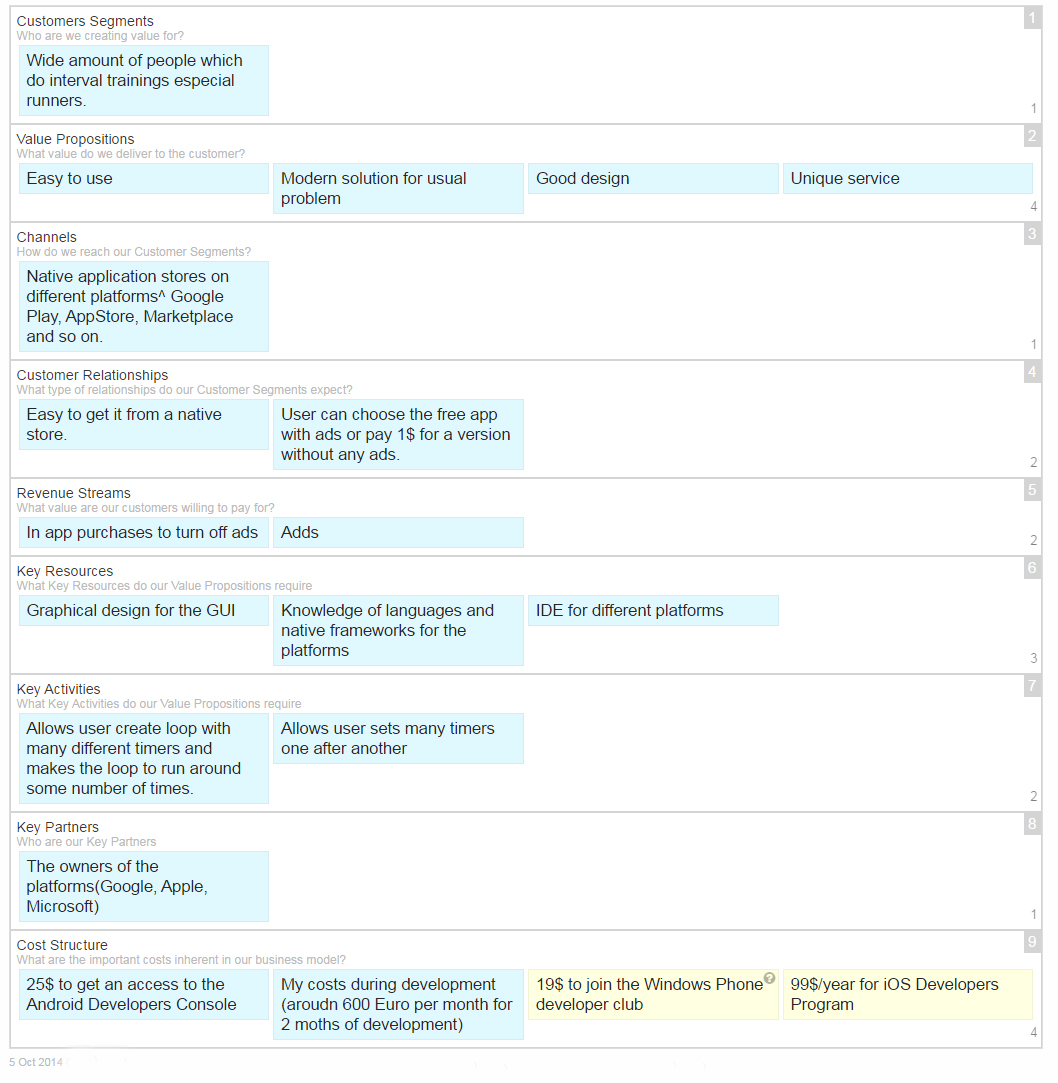
\includegraphics[scale=0.45]{BMC.jpg}

%MAIN CONTENT ******************************************************************************************************************


\end{document}
